\documentclass[]{article}
\usepackage{lmodern}
\usepackage{amssymb,amsmath}
\usepackage{ifxetex,ifluatex}
\usepackage{fixltx2e} % provides \textsubscript
\ifnum 0\ifxetex 1\fi\ifluatex 1\fi=0 % if pdftex
  \usepackage[T1]{fontenc}
  \usepackage[utf8]{inputenc}
\else % if luatex or xelatex
  \ifxetex
    \usepackage{mathspec}
  \else
    \usepackage{fontspec}
  \fi
  \defaultfontfeatures{Ligatures=TeX,Scale=MatchLowercase}
\fi
% use upquote if available, for straight quotes in verbatim environments
\IfFileExists{upquote.sty}{\usepackage{upquote}}{}
% use microtype if available
\IfFileExists{microtype.sty}{%
\usepackage{microtype}
\UseMicrotypeSet[protrusion]{basicmath} % disable protrusion for tt fonts
}{}
\usepackage[margin=1in]{geometry}
\usepackage{hyperref}
\hypersetup{unicode=true,
            pdftitle={Modeling latent changes in COVID-19 transmission over time},
            pdfauthor={Andrew Tredennick},
            pdfborder={0 0 0},
            breaklinks=true}
\urlstyle{same}  % don't use monospace font for urls
\usepackage{longtable,booktabs}
\usepackage{graphicx,grffile}
\makeatletter
\def\maxwidth{\ifdim\Gin@nat@width>\linewidth\linewidth\else\Gin@nat@width\fi}
\def\maxheight{\ifdim\Gin@nat@height>\textheight\textheight\else\Gin@nat@height\fi}
\makeatother
% Scale images if necessary, so that they will not overflow the page
% margins by default, and it is still possible to overwrite the defaults
% using explicit options in \includegraphics[width, height, ...]{}
\setkeys{Gin}{width=\maxwidth,height=\maxheight,keepaspectratio}
\IfFileExists{parskip.sty}{%
\usepackage{parskip}
}{% else
\setlength{\parindent}{0pt}
\setlength{\parskip}{6pt plus 2pt minus 1pt}
}
\setlength{\emergencystretch}{3em}  % prevent overfull lines
\providecommand{\tightlist}{%
  \setlength{\itemsep}{0pt}\setlength{\parskip}{0pt}}
\setcounter{secnumdepth}{0}
% Redefines (sub)paragraphs to behave more like sections
\ifx\paragraph\undefined\else
\let\oldparagraph\paragraph
\renewcommand{\paragraph}[1]{\oldparagraph{#1}\mbox{}}
\fi
\ifx\subparagraph\undefined\else
\let\oldsubparagraph\subparagraph
\renewcommand{\subparagraph}[1]{\oldsubparagraph{#1}\mbox{}}
\fi

%%% Use protect on footnotes to avoid problems with footnotes in titles
\let\rmarkdownfootnote\footnote%
\def\footnote{\protect\rmarkdownfootnote}

%%% Change title format to be more compact
\usepackage{titling}

% Create subtitle command for use in maketitle
\providecommand{\subtitle}[1]{
  \posttitle{
    \begin{center}\large#1\end{center}
    }
}

\setlength{\droptitle}{-2em}

  \title{Modeling latent changes in COVID-19 transmission over time}
    \pretitle{\vspace{\droptitle}\centering\huge}
  \posttitle{\par}
    \author{Andrew Tredennick}
    \preauthor{\centering\large\emph}
  \postauthor{\par}
      \predate{\centering\large\emph}
  \postdate{\par}
    \date{06 May, 2020}

\usepackage{float}

\begin{document}
\maketitle

\hypertarget{overview}{%
\subsection{Overview}\label{overview}}

The current \emph{Georgia stochostic model} of COVID-19 tranmission
incorporates a metric of human movement (\(\phi(t)\)) that moderates the
baseline tranmission rate (\(\beta\)): \(\beta(t) = \phi(t)\beta\). This
formulation is meant to represent the impact of social distancing.
Social distancing, while powerful, is not the only practice that can
reduce transmission. Other practices, such as wearing face coverings,
maintaining social distance in public spaces, and enhanced cleaning
practices, can also reduce transmission. These practices are difficult
to quantify in data and, in turn, are difficult to model explicitly.
Nonetheless, we expect that mobility data will become less informative
of transmission over time and that other practices will play a larger
role.

I used a basis function approach (spline modeling) to model a latent
temporal process that mediates baseline tranmission rate. The idea is to
include a smooth temporal function in the model that stands in for all
unobserved processes that can reduce transmission.

\hypertarget{implementation}{%
\subsection{Implementation}\label{implementation}}

We currently model the force of infection (\(f\)) at time \(t\) as:

\[
f(t) = \phi(t)\frac{\beta}{N} (I(t)),
\]

where, for simplicity, \(I\) stands for all infectious individuals at
time \(t\). The mobility index \(\phi\) looks like this:

\includegraphics{spline-report_files/figure-latex/phi-1}

I proposed to add a temporal basis function to incorporate additional
tranmission reduction over time that we cannot observe. Let the new
temporal term be \(\psi\), which is modeled as:

\[
\text{logit}\left(\psi(t)\right) = \sum_{i=1}^K q_i \xi_{i_t},
\]

where \(K\) is the number of knots, \(\mathbf{q}\) is a vector of spline
coefficients (to be fitted), and \(\mathbf{\xi}\) is a matrix basis
functions. I define the number of knots (\(K\)) as the number of days in
the data set divided by 7 (so, one knot per week). Note the logit
transformation to go from the linear scale to the 0 - 1 scale. Thus,
\(f(t)\) becomes: \(f(t) = \psi(t)\phi(t)\frac{\beta}{N} (I(t))\).

Assuming \(K = 9\), the basis functions are:

\includegraphics{spline-report_files/figure-latex/bfuncs-1}

Assuming a vector of \(\mathbf{q}\) values drawn from a normal
distribution with mean 0 and unit variance, the resulting function can
look like this:

\includegraphics{spline-report_files/figure-latex/bfuncfunc-1}

Using MIF, we actually fit the \(\mathbf{q}\) values to find the best
\(\psi\) trend.

\hypertarget{results}{%
\subsection{Results}\label{results}}

I fit two models to data through May 3, 2020, one model with the new
basis function and one without. Here are the data:

\includegraphics{spline-report_files/figure-latex/data-1}

The fitted spline coefficients produce a trend over time, which I plot
with the mobility trend and their combined influence on tranmission.
Recall that ``phi'' is the mobility metric and ``psi'' is the latent
metric produced by the spline fit.

\includegraphics{spline-report_files/figure-latex/trendfit-1}

And here are the two model fits. Note that both models include the
mobility covariate; the ``spline'' model also includes the spline fit
which additionaly augments the transmission rate (thick line in the
figure above).

\hypertarget{with-spline}{%
\subsubsection{With spline}\label{with-spline}}

\begin{figure}[!H]
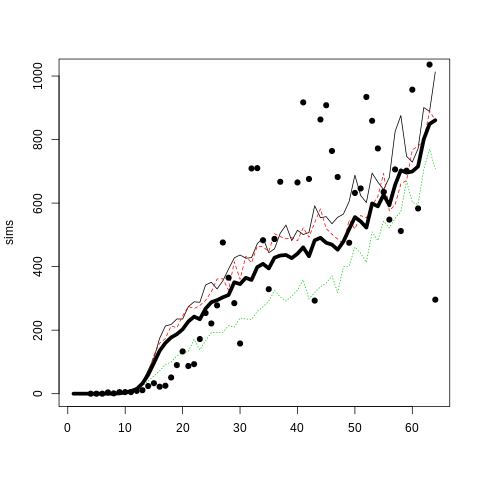
\includegraphics[width=0.75\linewidth,]{nospline} \caption{Fit of model to data with the spline for tranmission reduction (cases)}\label{fig:fig1}
\end{figure}

\hypertarget{without-spline}{%
\subsubsection{Without spline}\label{without-spline}}

\begin{figure}[!H]
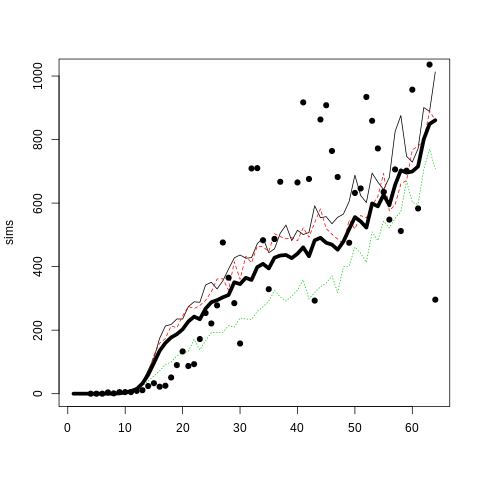
\includegraphics[width=1\linewidth,]{nospline} \caption{Fit of model to data with no spline for tranmission reduction (cases)}\label{fig:fig2}
\end{figure}

\hypertarget{model-comparison}{%
\subsubsection{Model comparison}\label{model-comparison}}

Here I compare the models via log likelihood and AIC. Note that for AIC
I just assume that the no spline mode has 0 parameters and that the
spline model has 9 paramters. This gets at the relative difference
between the two: the nine basis function coefficients.

\begin{longtable}[]{@{}lrr@{}}
\toprule
Model & Log Likelihood & AIC\tabularnewline
\midrule
\endhead
Without Spline & -800.8172 & 1601.634\tabularnewline
WIth Spline & -792.1416 & 1602.283\tabularnewline
\bottomrule
\end{longtable}

\hypertarget{discussion}{%
\subsection{Discussion}\label{discussion}}

Both models are equivalent according to AIC; judging be log likelihood
alone, the ``with spline'' model is superior. The two models lead to
rather different trajectories. The ``with spline'' model suggests a
flattening of the curve. The ``no spline'' model (which is the default)
suggests a continual growth in number of cases.

I think the real question is whether we ``buy'' the resulting trend
suggested by the fitted model in terms of how \(\beta\) is modulated by
mobility data and the latent process.


\end{document}
